%!TEX root = CooperBarba-orientation.tex

The results detailed in this section were obtained using an extension of the open-source code \pygbe,\footnote{\href{https://github.com/barbagroup/pygbe}{https://github.com/barbagroup/pygbe}} accounting for the presence of surfaces with imposed charge or potential.\cite{CooperBarba2015a}
We ran the calculations for protein \gb on a workstation with Intel Xeon X5650 \cpu s  and one \nvidia Tesla C2075 \gpu\ card (late 2011). 
The final case considers the antibody immunoglobulin G, which is a much larger molecule than protein \gb. For these runs, we used Boston University's \textsc{bungee} cluster, which has 16 nodes with 8 Intel Xeon \cpu\ cores each, and a total of 3 \nvidia Tesla Kepler K20 (late 2012) and 26 \nvidia Tesla M2070/2075 \gpu s. All runs were serial: single-\cpu\ and single-\gpu. 
We obtained the van der Waals radii and charge distribution using \texttt{pdb2pqr}\cite{Dolinsky04} with an \amber forcefield, and generated the meshes using the free \msms software.\cite{SannerOlsonSpehner1995}
In these tests, we did not consider a Stern layer for either the protein or the charged surface, nor the presence of solvent-filled cavities inside the protein.

\subsection{First case: protein G\,B1\,D4$^{\prime}$} \label{sec:PGB}

We investigated the preferred orientation of protein \gb placed 2\AA\ away from a 100\AA$\times$100\AA$\times$10\AA\ block with surface charge density $\pm$0.05C/m$^2$, centered with respect to a 100\AA$\times$100\AA\ face.
In biosensors, protein \gb can be used as an intermediate protein, coupled to the functionalized surface directly by covalent bonding.
The protein will thus be at a small distance from the surface. In this case, 2\AA\ is in the order of magnitude of the size of a water molecule, or of a C--N bond.
The charge density of $\pm$0.05C/m$^2$ matches that used in other works.\cite{LiuLiaoZhou2013}
In these cases, we considered a solvent with no salt, i.e., $\kappa=0$ (to compare with other published results), and with relative permittivity 80. The region inside the protein had a relative permittivity of 4.

As seen in Figure \ref{fig:1pgb_orientation}, $\alpha_\text{tilt}$ is the angle between the protein's dipole moment and the normal vector to the surface, and $\alpha_\text{rot}$ rotates about the dipole moment. 
When the dipole-moment vector and the normal are aligned ($\alpha_\text{rot}=0$), we define a vector $\mathbf{V}_\text{ref}$ as the shortest distance between the axis normal to the surface that goes through the center of mass, and the atom that is furthest away from it. 
We use $\mathbf{V}_\text{ref}$ as a reference to define the rotation angle $\alpha_\text{rot}$: the angle between $\mathbf{V}_\text{ref}$ and the vector normal to a 100\AA$\times$10\AA\ face.  


We sampled the total free energy every $\Delta \alpha_{\text{tilt}} = 2^\circ$ of tilt angle and $\Delta \alpha_{\text{rot}} =10^\circ$ of rotation angle, resulting in $3,240$ independent runs.  The surface mesh had 4 triangles per square Angstrom on the protein geometry and 2 triangles per square Angstrom on the charged surface. 

Numerical parameters are presented in Table \ref{table:params3}. In a companion publication,\cite{CooperBarba2015a} we present a grid-convergence study using both an analytical solution and a case with protein \gb.\cite{CooperBarba2015-share1348803} We computed an approximate exact value of $-222.43$[kcal/mol] for solvation energy and $317.98$[kcal/mol] for surface energy using Richardson extrapolation with very fine parameters. With results that are less than 2\% away from the approximate exact values, we are comfortable with the parameters in Table \ref{table:params3} and mesh densities of $4$ elements per square Angstrom on the protein and $2$ elements per square Angstrom on the surface.\cite{CooperBarba2015a}

\begin{table}[h]
  %\centering
   %\fontfamily{ppl}\selectfont
   \caption{\label{table:params3}Numerical parameters used for numerically probing the orientation of protein \gb. } 
    \begin{tabular}{c c c c c c c}
	\hline%\toprule
	\multicolumn{3}{l} {\# Gauss points:} & \multicolumn{3}{l}{Treecode:} & \gmres:\\
	\footnotesize{in-element} & \footnotesize{close-by} & \footnotesize{far-away} & $N_{\text{crit}}$ & $P$ &  $\theta$  & tol.\\
	\hline%\midrule
	9 per side & 19 & 1  &  300 & 4 & 0.5  & $10^{-5}$\\	
	\hline%\bottomrule
    \end{tabular}
\end{table}

Using total free energy as the input, the integrals of Equation \eqref{eq:prob_angle} can be computed by means of the trapezoidal rule. Figure \ref{fig:1PGB_probability} presents the probability of the protein orientation in terms of $\cos(\alpha_{\text{tilt}})$, in intervals of $\Delta \cos(\alpha_{\text{tilt}}) = 0.005$ (Fig.~\ref{fig:1PGB_cos}) and $\Delta \alpha_{\text{tilt}}$=2$^{\circ}$ (Fig.~\ref{fig:1PGB_alpha}). Table \ref{table:avg} presents the average orientation $<\cos(\alpha_{\text{tilt}})>$ for the surface having either positive or negative charge density, and Figure \ref{fig:field} shows the electrostatic potential for the preferred orientation in each case. 

\begin{figure*}
   \centering
   \subfloat[]{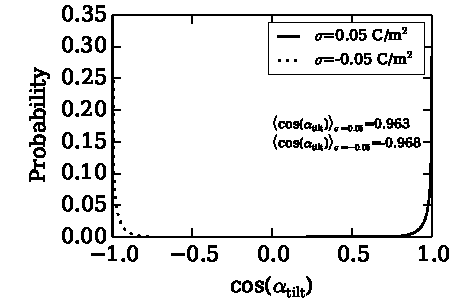
\includegraphics[width=0.43\textwidth]{Figure5a.pdf} \label{fig:1PGB_cos}}
   \subfloat[]{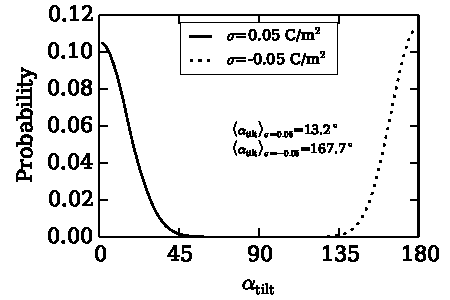
\includegraphics[width=0.43\textwidth]{Figure5b.pdf} \label{fig:1PGB_alpha}}\\
   \subfloat[]{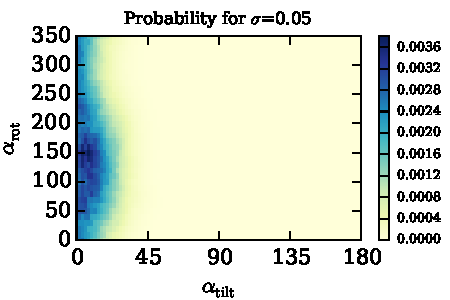
\includegraphics[width=0.40\textwidth]{Figure5c.pdf} \label{fig:1PGB_2D_sig005}}
   \subfloat[]{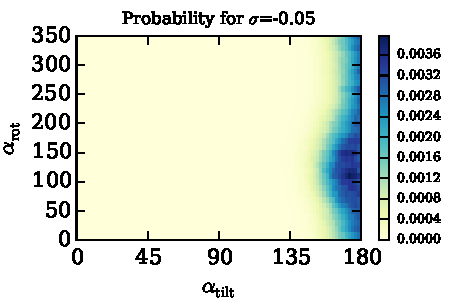
\includegraphics[width=0.40\textwidth]{Figure5d.pdf} \label{fig:1PGB_2D_sig-005}}
   \caption{Orientation probability distribution of protein \gb. Figures \ref{fig:1PGB_cos} and \ref{fig:1PGB_alpha} are the probability with respect to the tilt angle and its cosine, respectively. Figures \ref{fig:1PGB_2D_sig005} and \ref{fig:1PGB_2D_sig-005} are the probability distributions with respect to both the tilt and rotation angles. Data sets, figure files and running/plotting scripts are available under \ccby.\cite{CooperBarba2015-share1348804}}
   \label{fig:1PGB_probability}
\end{figure*}

\begin{table}[h]
   \caption{\label{table:avg}Average orientation.} 
    \begin{tabular}{c c}
	\hline
	\multicolumn{2}{c} {$<\cos(\alpha_{\text{tilt}})>$} \\
	Negative & Positive \\
	\hline
	$-0.968$ & $0.963$ \\	
	\hline
    \end{tabular}
\end{table}

\begin{figure*}
   \centering
   \subfloat[Negative surface charge ($\alpha_\text{tilt}=172^\circ$, $\alpha_\text{rot}=110^\circ$)]{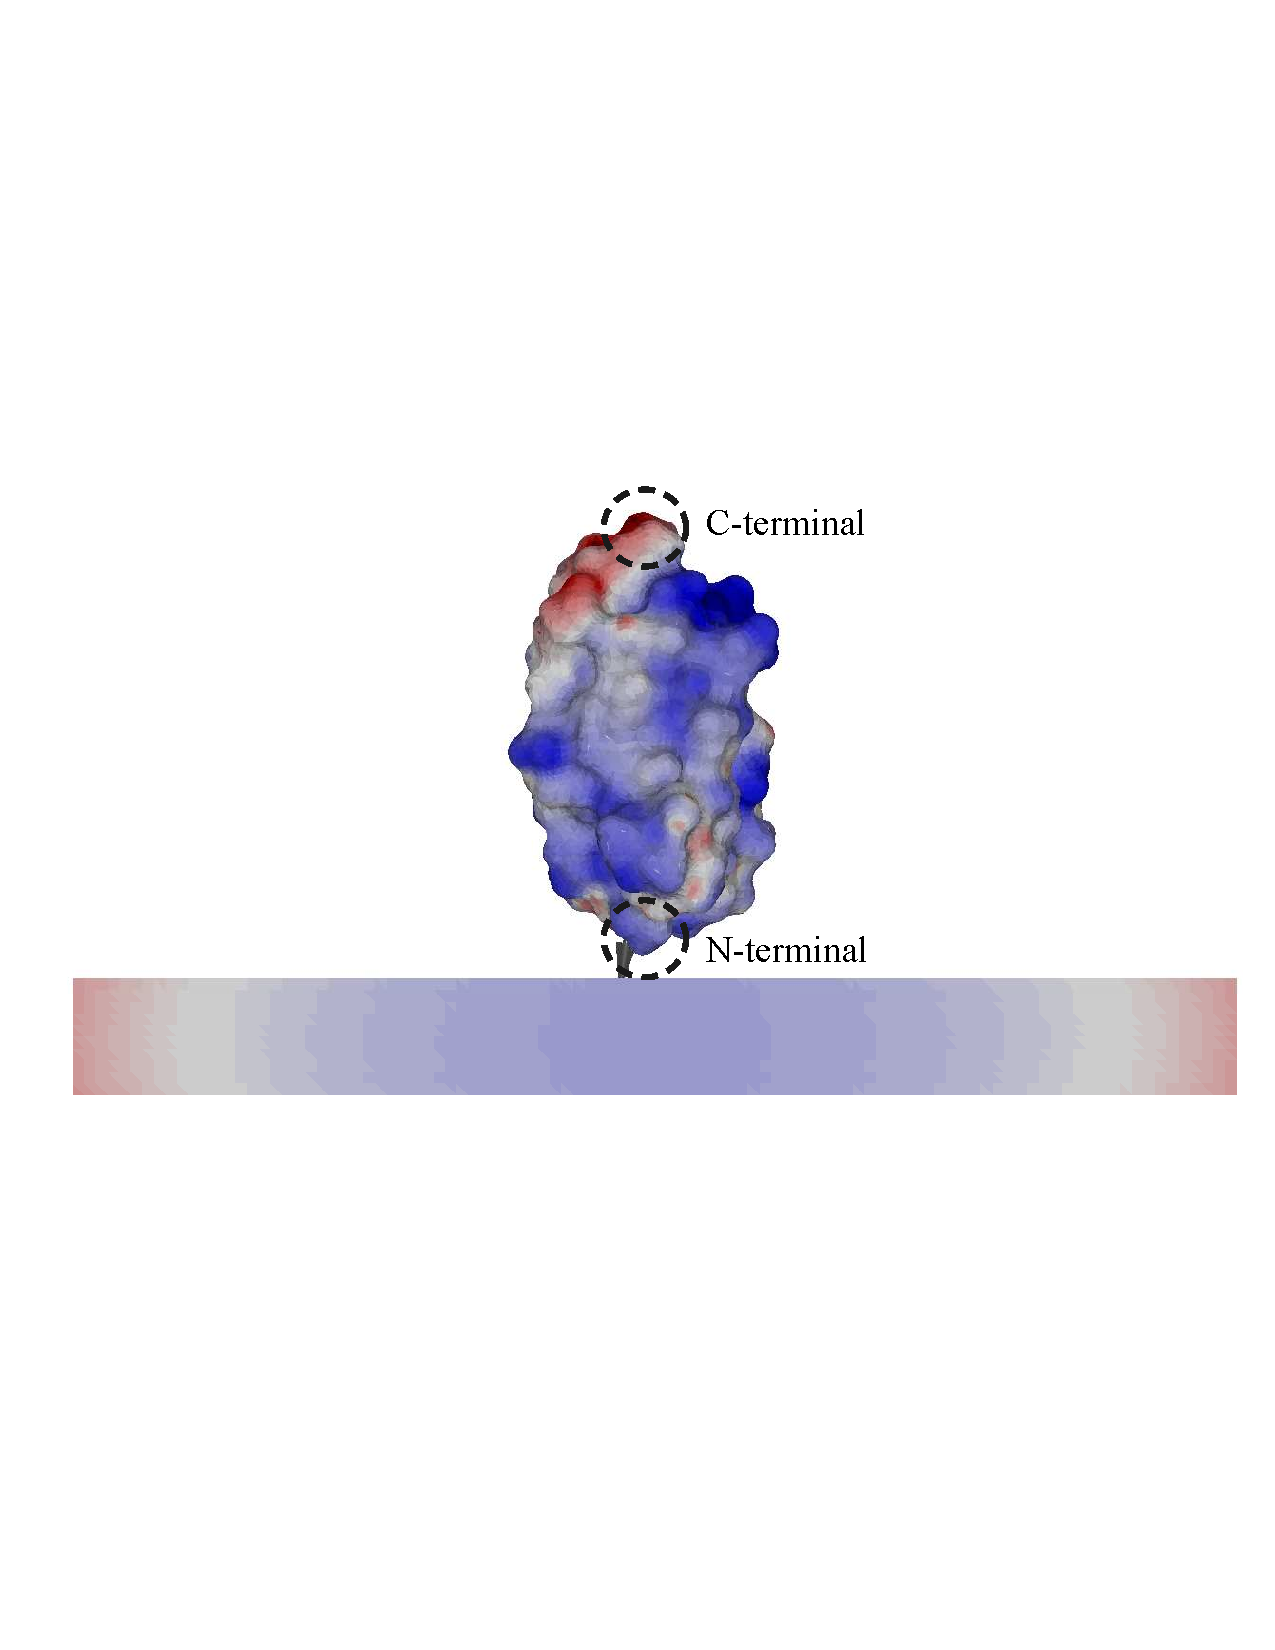
\includegraphics[width=0.48\textwidth]{Figure6a.pdf} \label{fig:phi_sig-0.05}} 
   \subfloat[Positive surface charge ($\alpha_\text{tilt}=8^\circ$, $\alpha_\text{rot}=150^\circ$)]{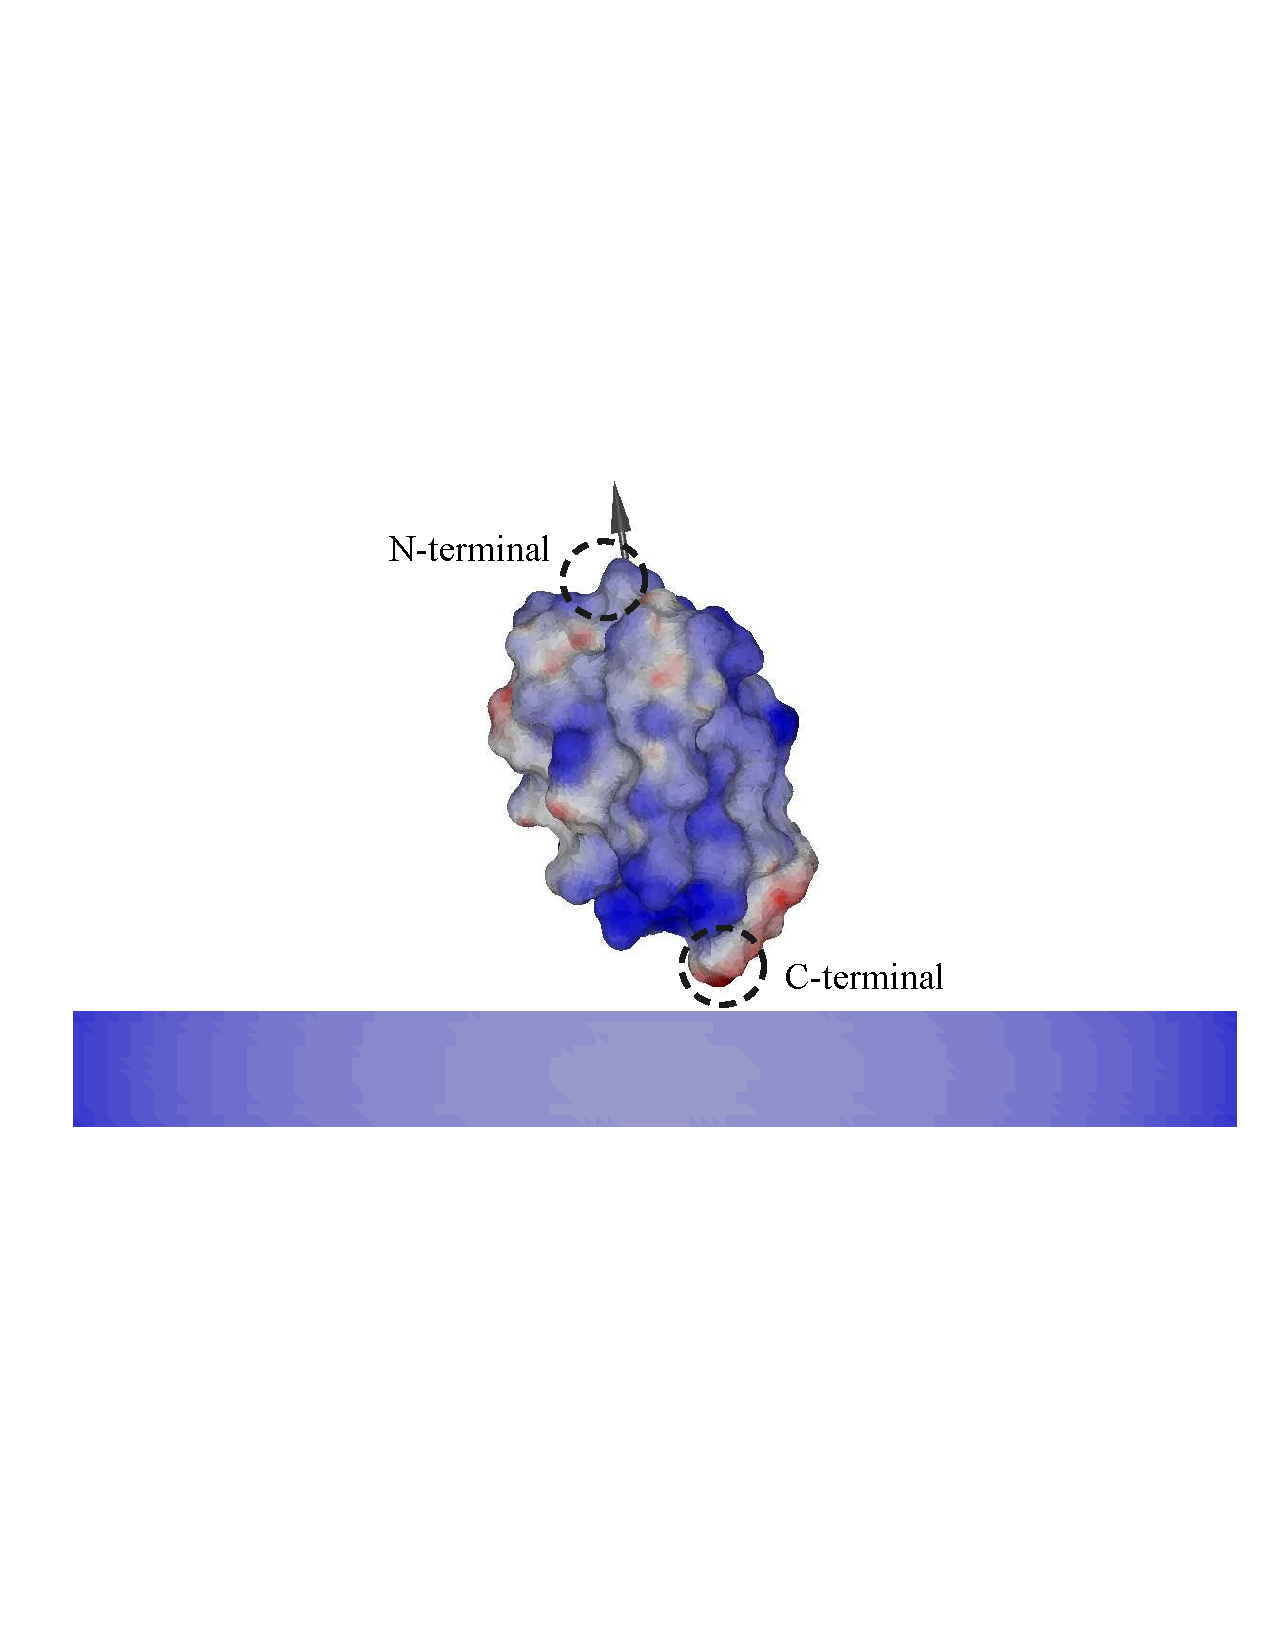
\includegraphics[width=0.48\textwidth]{Figure6b.pdf} \label{fig:phi_sig0.05}} 
   \caption{Electrostatic potential of protein \gb for the preferred orientations according to Figure \ref{fig:1PGB_probability}. Black arrow indicates direction of dipole-moment vector.}
   \label{fig:field}
\end{figure*}

\subsection{Second case: immunoglobulin G} \label{sec:IGT}


We computed the electrostatic field of immunoglobulin G---a protein widely used in biosensors---interacting with a 250\AA$\times$250\AA$\times$10\AA\ block, varying the conditions of surface charge and salt concentration. The protein was centered with respect to a  250\AA$\times$250\AA\ face, at a distance 5\AA\ above it. 
In fabrication, antibodies are usually immobilized on the biosensor surface via a cross-linker molecule, which we model here by increasing the distance from the surface.
As before, the solvent had relative permittivity of 80 and the protein of 4.

\medskip

 \paragraph*{Grid-convergence study for immunoglobulin G---}

Since this was the first time we did calculations on immunoglobulin G, we carried out a grid-convergence study to make sure the geometry was well resolved and to find adequate values of the simulation parameters for sampling different orientations. The error plotted in Figure \ref{fig:1IGT_convergence} is the relative difference between the energy obtained using \pygbe with each mesh density and the estimated exact value computed with Richardson extrapolation.

In this case, we computed the solvation energy and surface energy of a system consisting of a surface with charge density 0.05C/m$^2$ and a protein with $\alpha_{\text{tilt}} = 31^{\circ}$ and $\alpha_{\text{rot}} = 130^{\circ}$. Using the results from runs with a mesh density of 2, 4, and 8 elements per square Angstrom, we added the solvation and surface energies, and used Richardson extrapolation to obtain a value of $-2792.22$[kcal/mol], and an \emph{observed order of convergence} of 0.85. This is our reference to calculate the errors in Figure \ref{fig:1IGT_convergence}. There is a slight deviation from the expected value of the observed order of convergence (1.0), which we attribute to the non-uniform mesh generated by \msms. Even though the mesh density is on average doubled for each run, there is no guarantee that the refinement is homogeneous throughout the whole molecular surface. The numerical parameters are presented in Table \ref{table:params4}.

\begin{table}[h]
  %\centering
   %\fontfamily{ppl}\selectfont
   \caption{\label{table:params4}Numerical parameters used in the grid-convergence study with immunoglobulin G. } 
    \begin{tabular}{c c c c c c c}
	\hline%\toprule
	\multicolumn{3}{l} {\# Gauss points:} & \multicolumn{3}{l}{Treecode:} & \gmres:\\
	\footnotesize{in-element} & \footnotesize{close-by} & \footnotesize{far-away} & $N_{\text{crit}}$ & $P$ &  $\theta$  & tol.\\
	\hline%\midrule
	9 per side & 19 & 1  &  1000 & 6 & 0.5  & $10^{-5}$\\	
	\hline%\bottomrule
    \end{tabular}
\end{table}




\begin{figure}[h] %  figure placement: here, top, bottom, or page
   \centering
   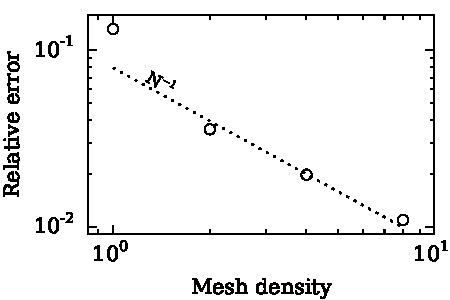
\includegraphics[width=0.45\textwidth]{Figure7.pdf} 
   \caption{Grid-convergence study of the solvation plus surface energy for immunoglobulin G interacting with a surface with charge density of 0.05C/m$^2$. Data sets, figure files and plotting scripts are available under \ccby.\cite{CooperBarba2015-share1348801}}
   \label{fig:1IGT_convergence}
\end{figure}



\medskip 

 \paragraph*{Probing orientation of immunoglobulin G---}

We sampled the total free energy every $\Delta \alpha_{\text{tilt}} = 4^\circ$ of tilt angle and $\Delta \alpha_{\text{rot}} =20^\circ$ of rotation angle, resulting in a total of 810 runs.  The surface meshes had 2 triangles per square Angstrom throughout. Numerical parameters are presented in Table \ref{table:params5}.

\begin{table}[h]
  %\centering
   %\fontfamily{ppl}\selectfont
   \caption{\label{table:params5}Numerical parameters used in the runs probing orientation of immunoglobulin G. } 
    \begin{tabular}{c c c c c c c}
	\hline%\toprule
	\multicolumn{3}{l} {\# Gauss points:} & \multicolumn{3}{l}{Treecode:} & \gmres:\\
	\footnotesize{in-element} & \footnotesize{close-by} & \footnotesize{far-away} & $N_{\text{crit}}$ & $P$ &  $\theta$  & tol.\\
	\hline%\midrule
	9 per side & 19 & 1  &  300 & 2 & 0.5  & $10^{-4}$\\	
	\hline%\bottomrule
    \end{tabular}
\end{table}

With the computed total free energy, we obtained the probability of each orientation using Equation \eqref{eq:prob_angle} and the trapezoidal rule.  
We sampled all combinations with surface charges of $\sigma=\pm$0.05C/m$^2$ and $\sigma = \pm$ 0.1C/m$^2$ and salt concentrations of 145mM ($\kappa$ = 0.125 \AA$^{-1}$) and 37mM ($\kappa$ = 0.0625 \AA$^{-1}$). For each of these cases, Figures \ref{fig:1IGT_negcharge}  and \ref{fig:1IGT_poscharge} show a color plot of the probability distribution with respect to the tilt and rotation angles, and a 3D plot of the preferred orientation, where the solvent-excluded surface is colored by the electrostatic potential.

% FIGURE 8
\begin{figure*} 
   \centering
   \subfloat[Probability for $\sigma=-0.05$C/m$^2$, $\kappa=0.125$\AA$^{-1}$]{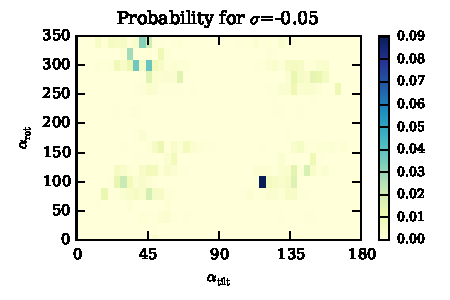
\includegraphics[width=0.4\textwidth]{Figure8a.pdf} \label{fig:1IGT_2D_sig-005}}
   \subfloat[x-y plane view for $\alpha_{\text{tilt}} = 116^{\circ}$ and $\alpha_{\text{rot}} = 100^{\circ}$]{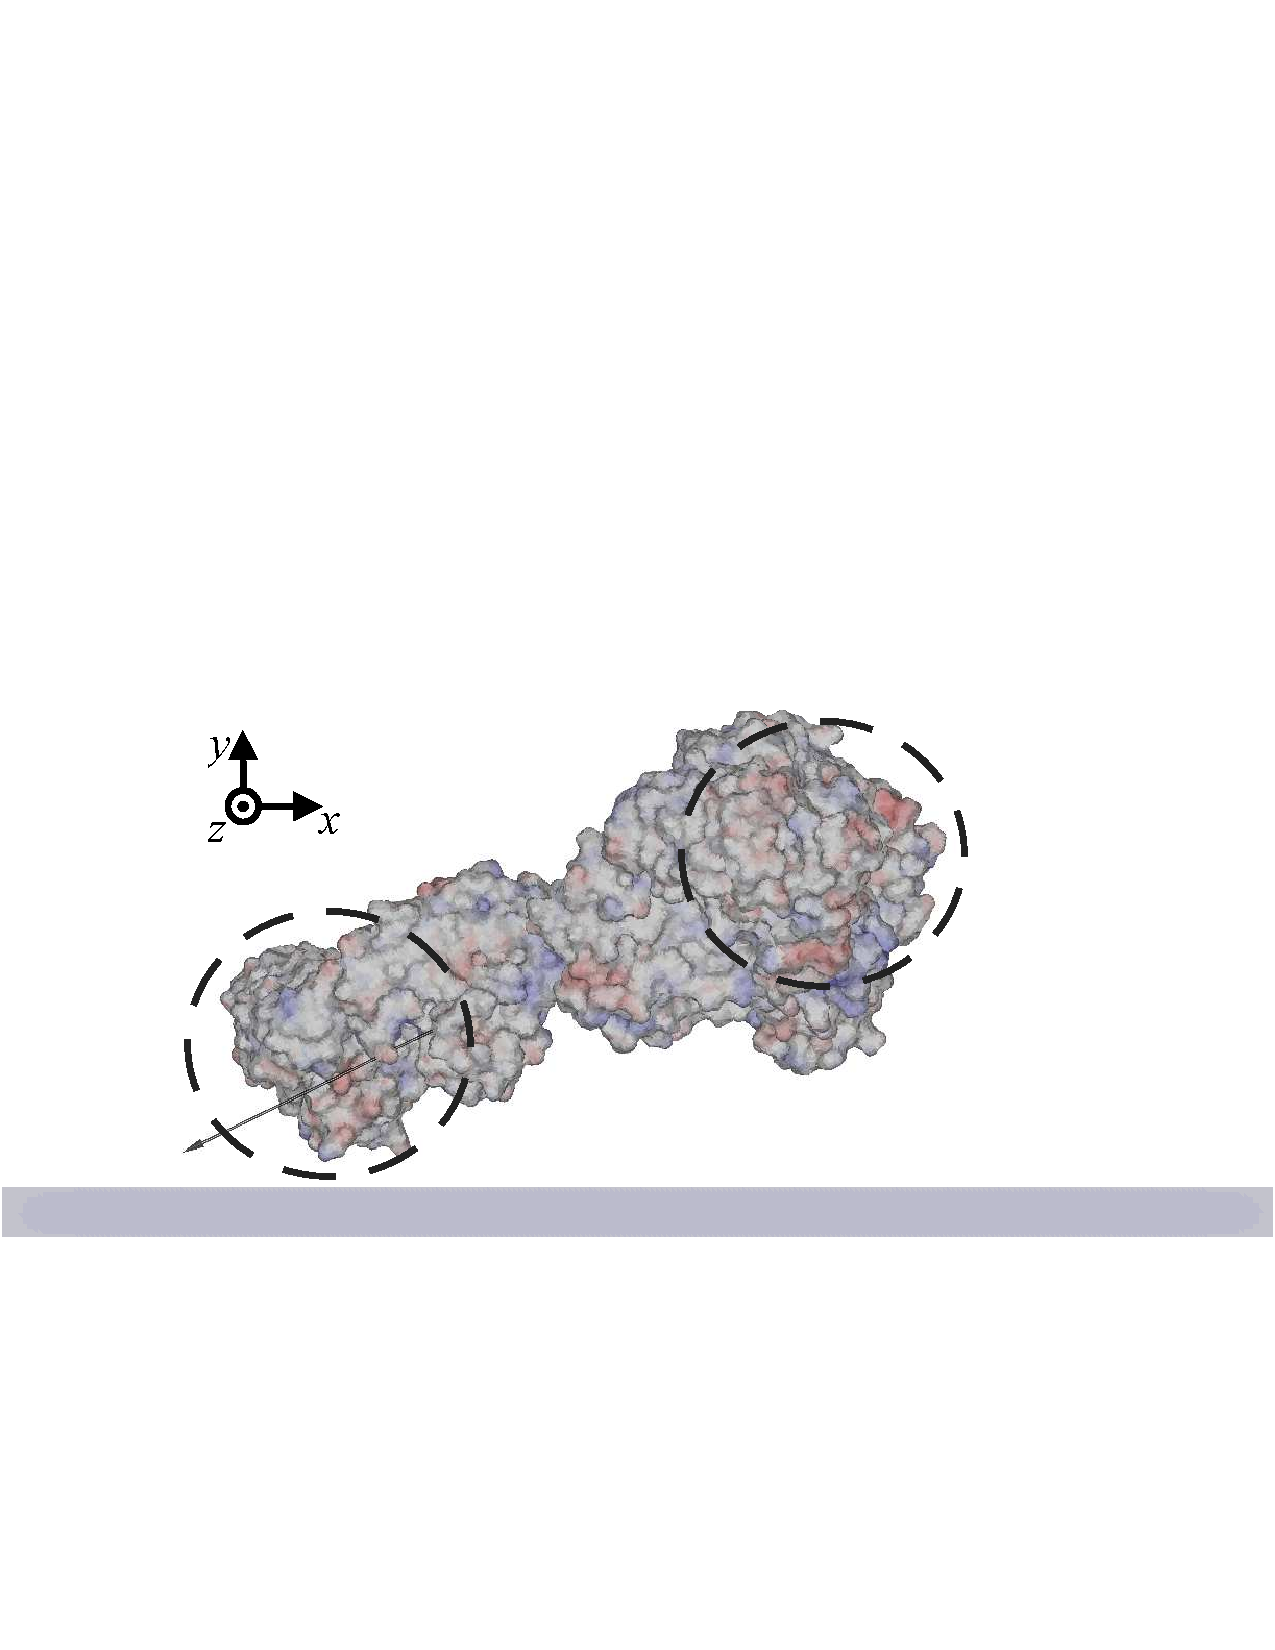
\includegraphics[width=0.4\textwidth]{Figure8b.pdf} \label{fig:1IGT_3D_sig-005_kap0125_til116-rot100}}\\
   \subfloat[Probability for $\sigma=-0.1$C/m$^2$, $\kappa=0.125$\AA$^{-1}$]{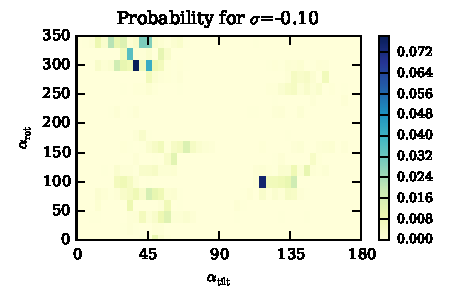
\includegraphics[width=0.4\textwidth]{Figure8c.pdf} \label{fig:1IGT_2D_sig-020_kappa01250}}
   \subfloat[y-z plane view for $\alpha_{\text{tilt}} = 36^{\circ}$ and $\alpha_{\text{rot}} = 300^{\circ}$]{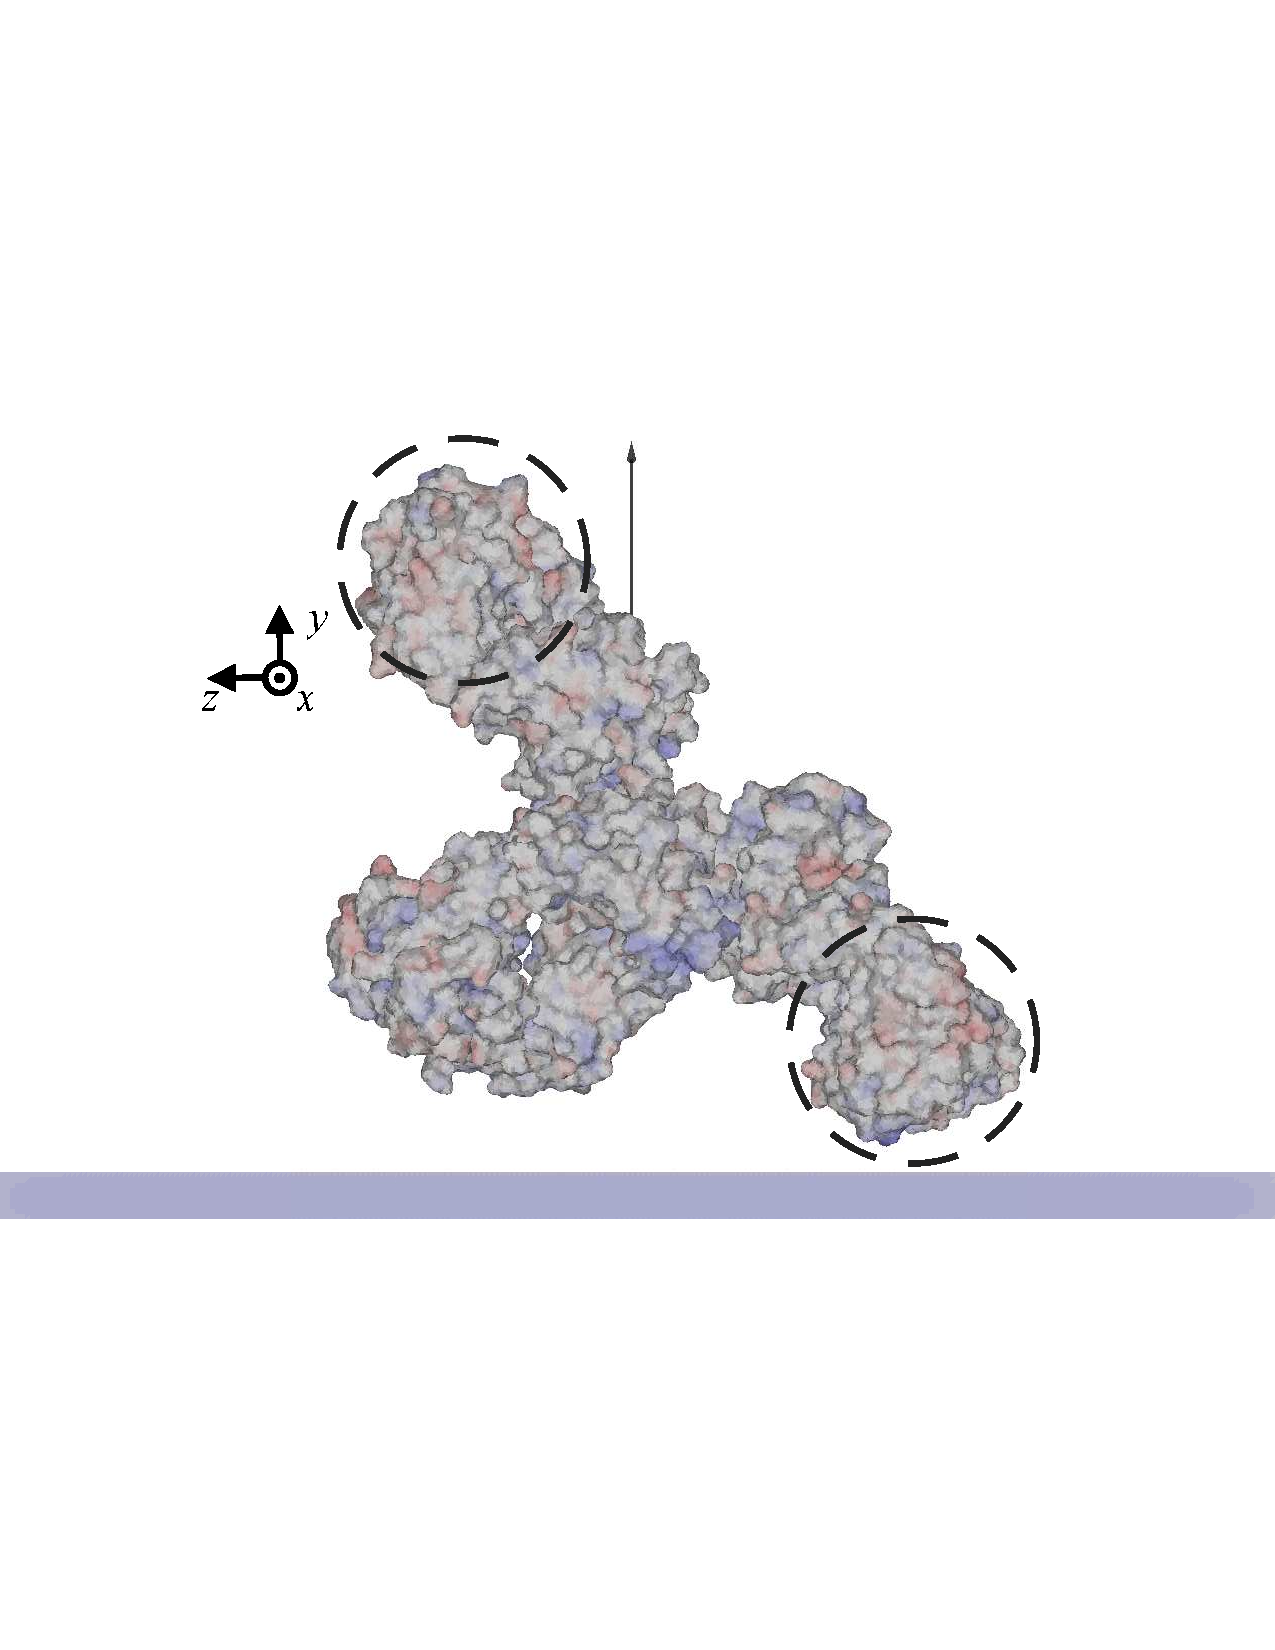
\includegraphics[width=0.4\textwidth]{Figure8d.pdf} \label{fig:1IGT_3D_sig-02_kap0125_til056-rot040}}\\
   \subfloat[Probability for $\sigma=-0.05$C/m$^2$, $\kappa=0.0625$\AA$^{-1}$]{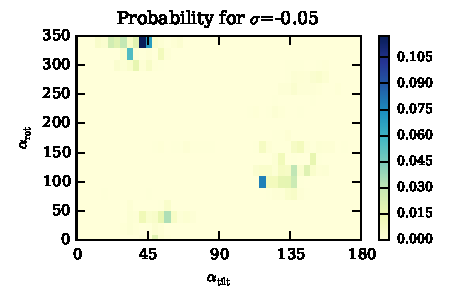
\includegraphics[width=0.4\textwidth]{Figure8e.pdf} \label{fig:1IGT_2D_sig-005_kappa003125}}
   \subfloat[x-y plane view for $\alpha_{\text{tilt}} = 40^{\circ}$ and $\alpha_{\text{rot}} = 340^{\circ}$]{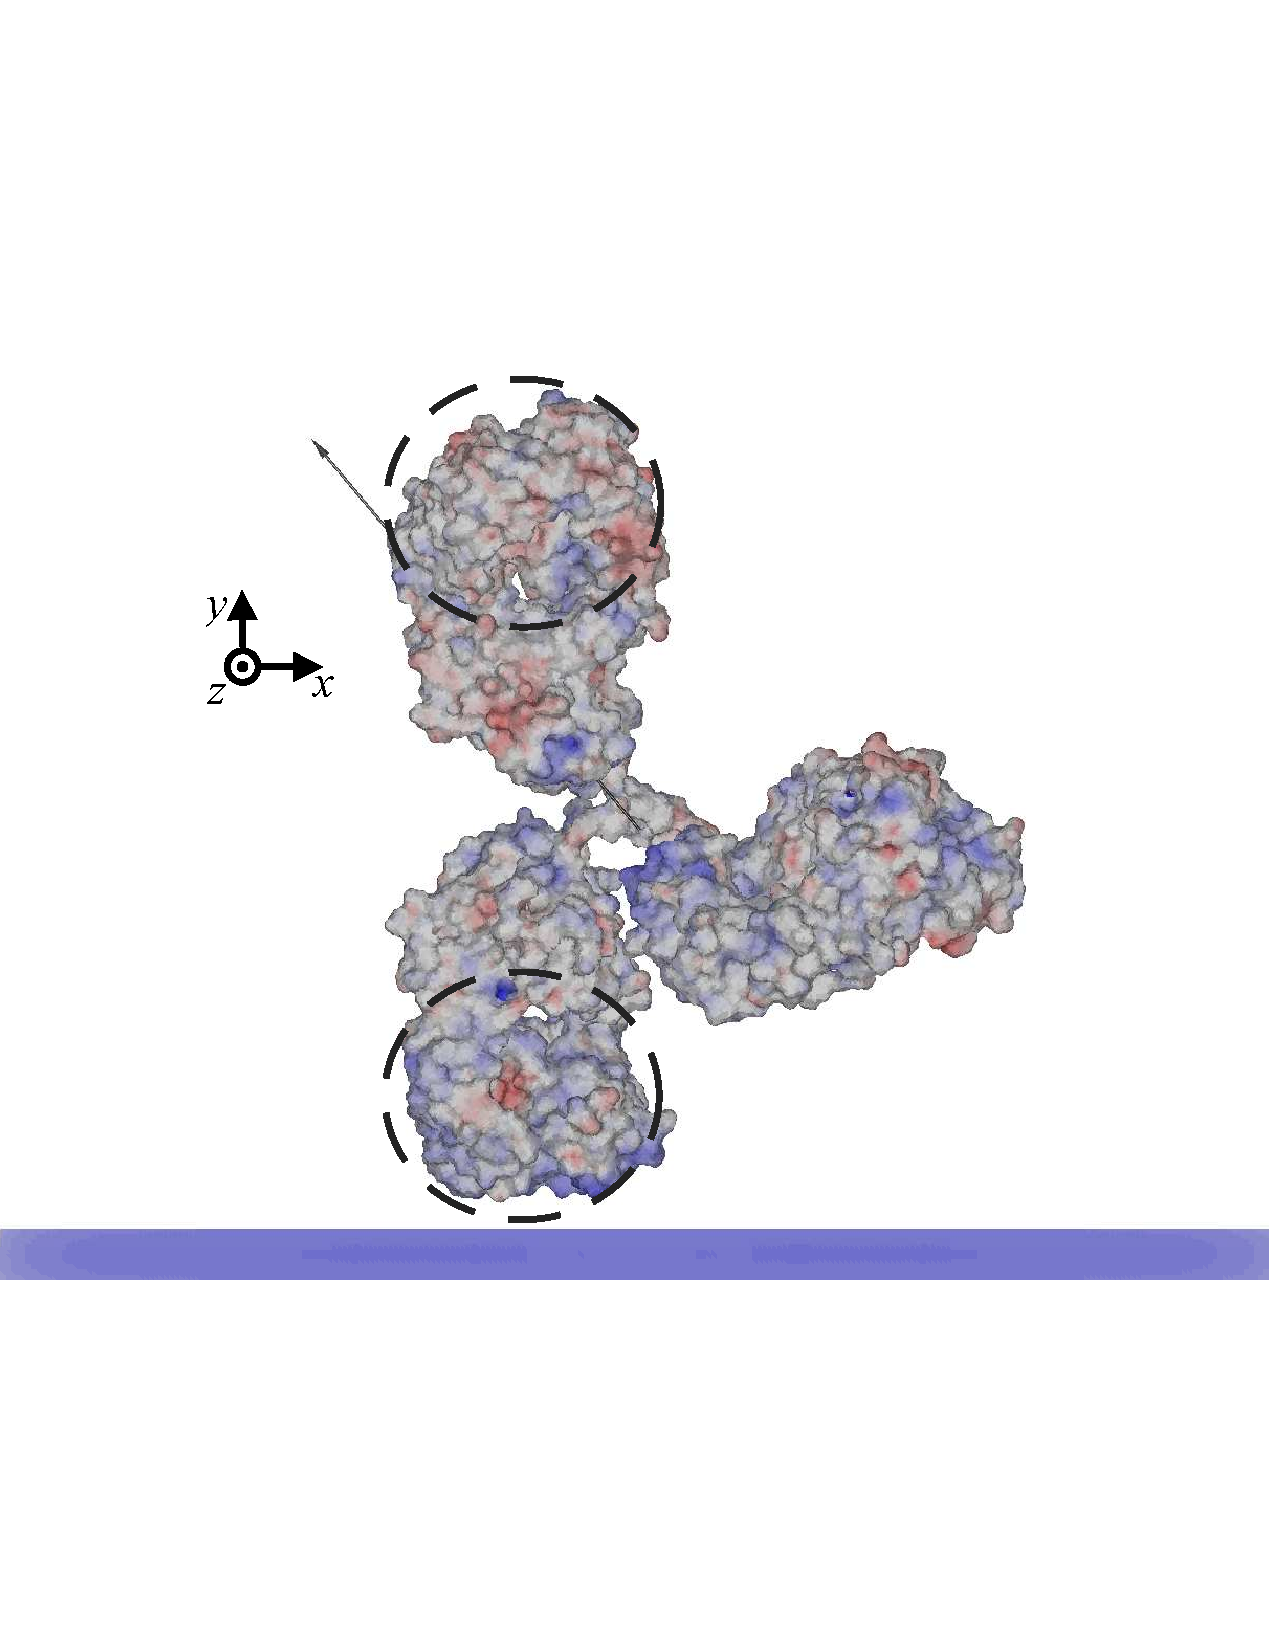
\includegraphics[width=0.4\textwidth]{Figure8f.pdf} \label{fig:1IGT_3D_sig-005_kap003125_til116-rot160}}\\
   \subfloat[Probability for $\sigma=-0.1$C/m$^2$, $\kappa=0.0625$\AA$^{-1}$]{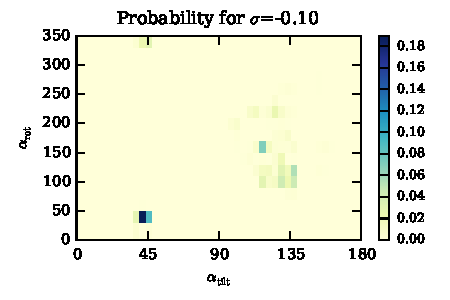
\includegraphics[width=0.4\textwidth]{Figure8g.pdf} \label{fig:1IGT_2D_sig-020_kappa003125}}
   \subfloat[x-y plane view for $\alpha_{\text{tilt}} = 40^{\circ}$ and $\alpha_{\text{rot}} = 40^{\circ}$]{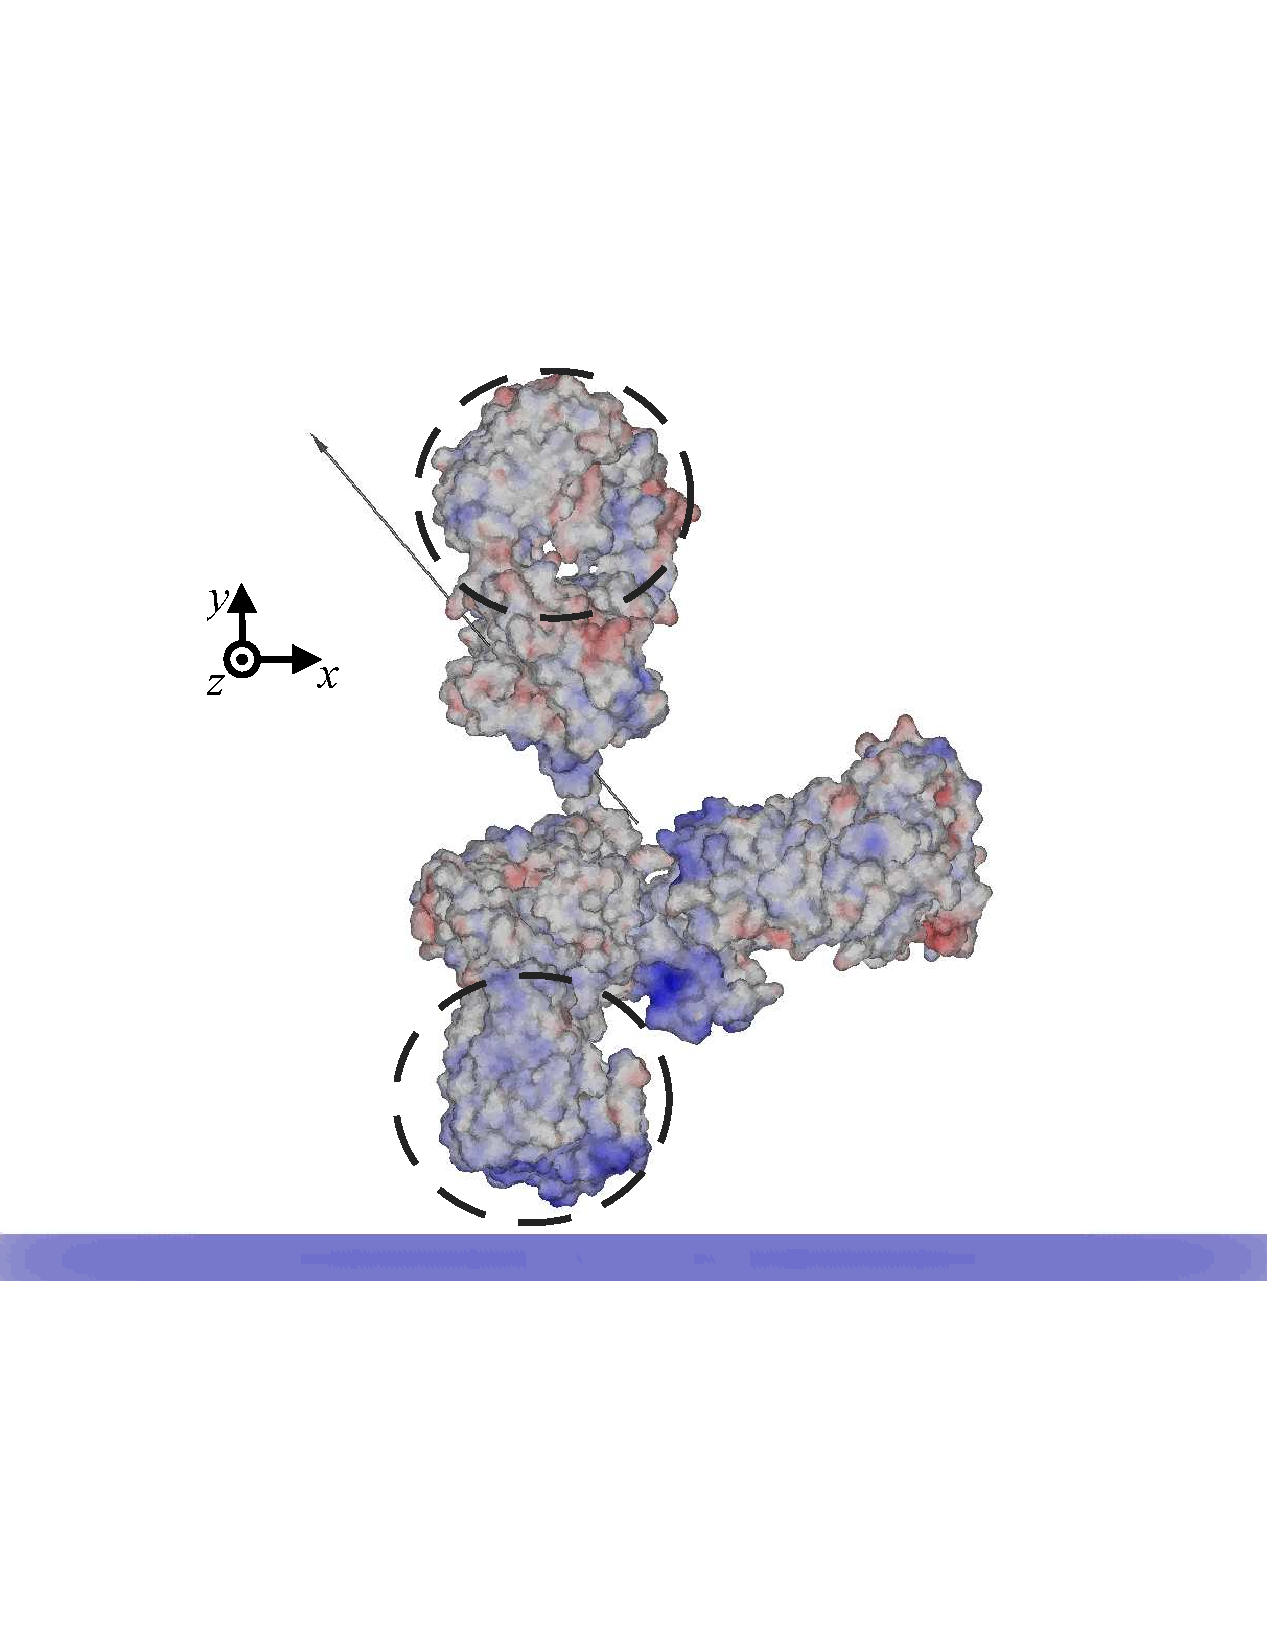
\includegraphics[width=0.4\textwidth]{Figure8h.pdf} \label{fig:1IGT_3D_sig-02_kap003125_til124-rot140}}
   \caption{Orientation probability distribution and surface potential of the preferred orientation for immunoglobulin G near a negative surface charge. The black arrow indicates the direction of the dipole moment, and the circles enclose the Fab fragments. Data sets, figure files and plotting scripts available under \ccby.\cite{CooperBarba2015-share1348802}}
   \label{fig:1IGT_negcharge}
\end{figure*}


\begin{figure*}
   \centering
   \subfloat[Probability for $\sigma$=0.05C/m$^2$ and $\kappa$=0.125\AA$^{-1}$]{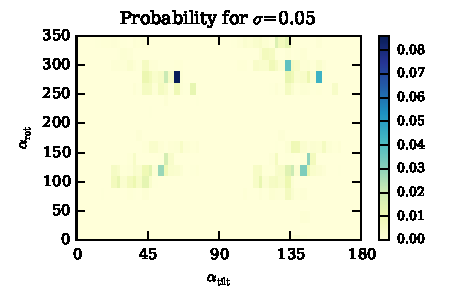
\includegraphics[width=0.4\textwidth]{Figure9a.pdf} \label{fig:1IGT_2D_sig005}}
   \subfloat[x-y plane view for $\alpha_{\text{tilt}} = 64^{\circ}$ and $\alpha_{\text{rot}} = 280^{\circ}$]{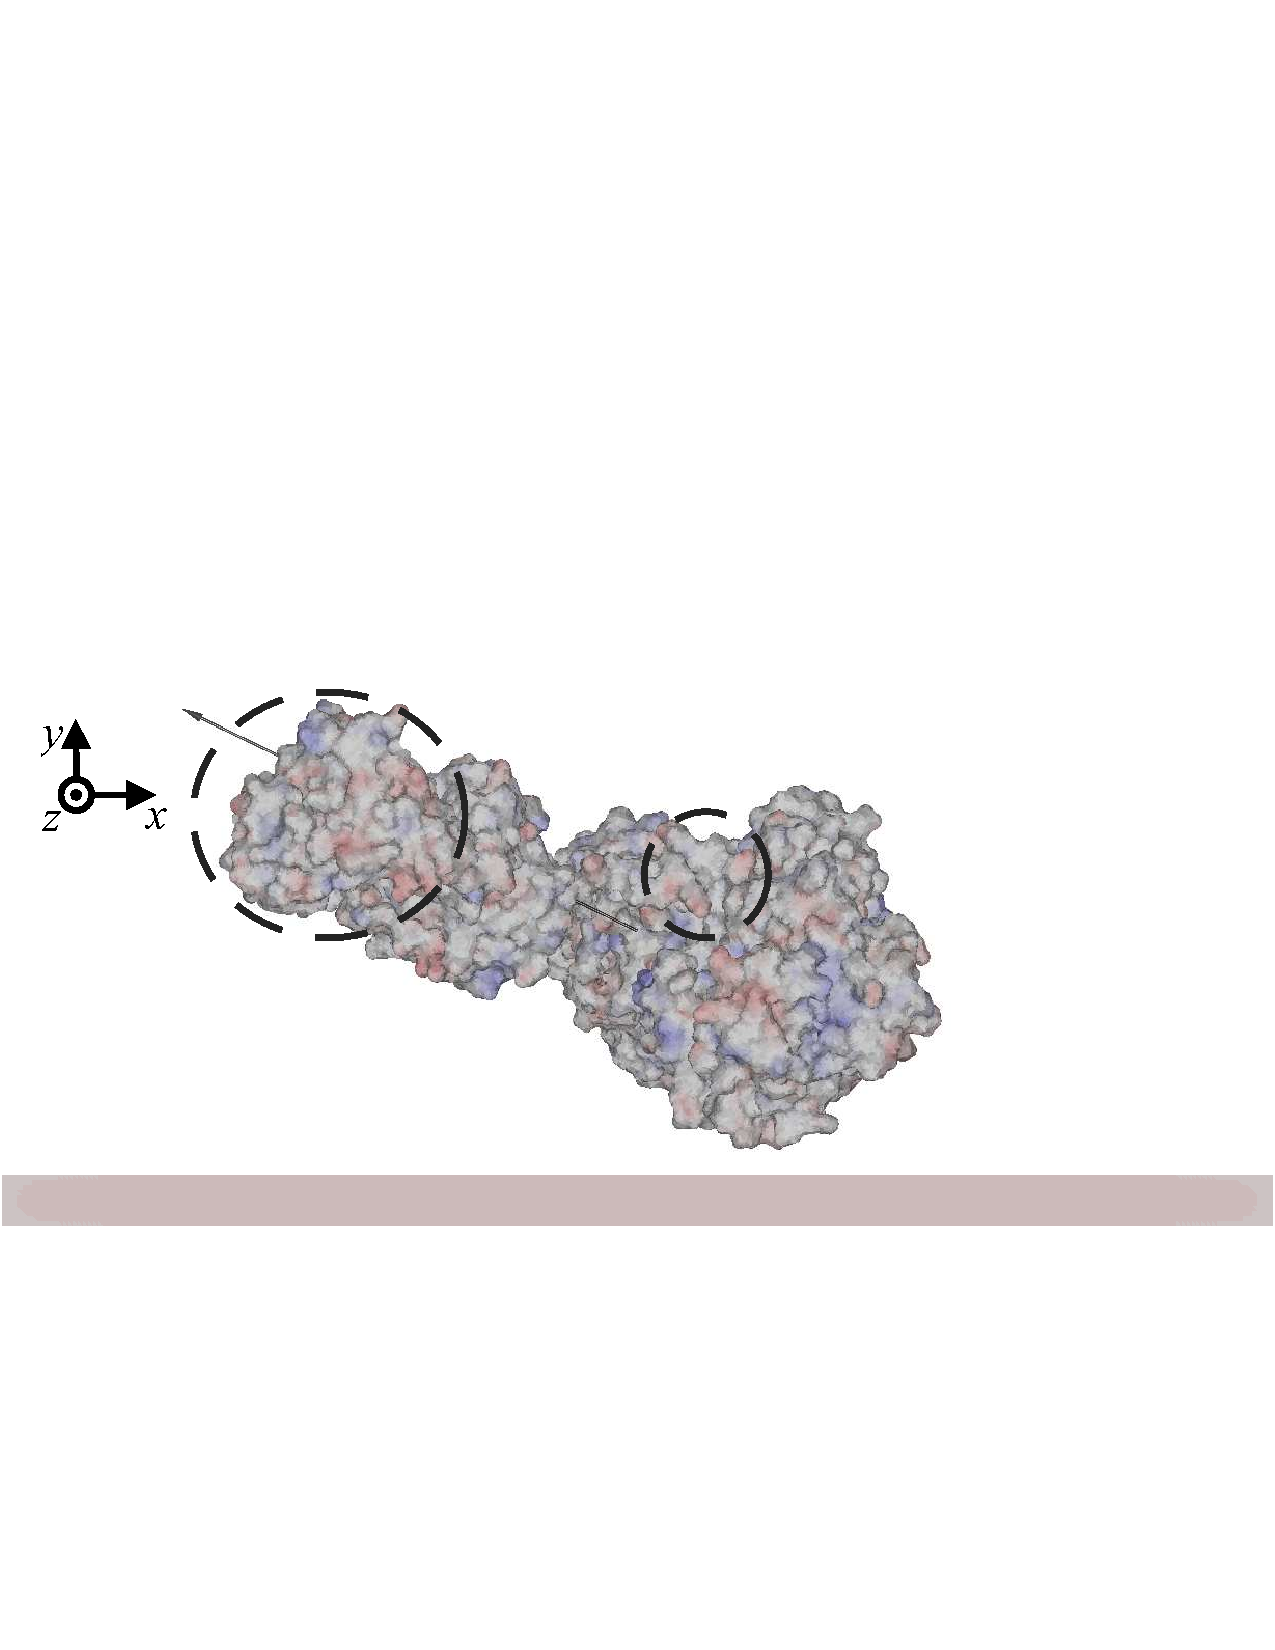
\includegraphics[width=0.4\textwidth]{Figure9b.pdf} \label{fig:1IGT_3D_sig005_kap0125_til064-rot280}}\\
   \subfloat[Probability for $\sigma$=0.1C/m$^2$ and $\kappa$=0.125\AA$^{-1}$]{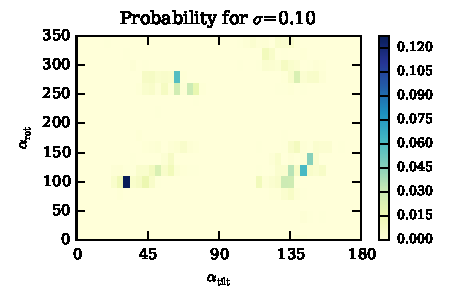
\includegraphics[width=0.4\textwidth]{Figure9c.pdf} \label{fig:1IGT_2D_sig020_kappa01250}}
   \subfloat[y-z plane view for $\alpha_{\text{tilt}} = 32^{\circ}$ and $\alpha_{\text{rot}} = 100^{\circ}$]{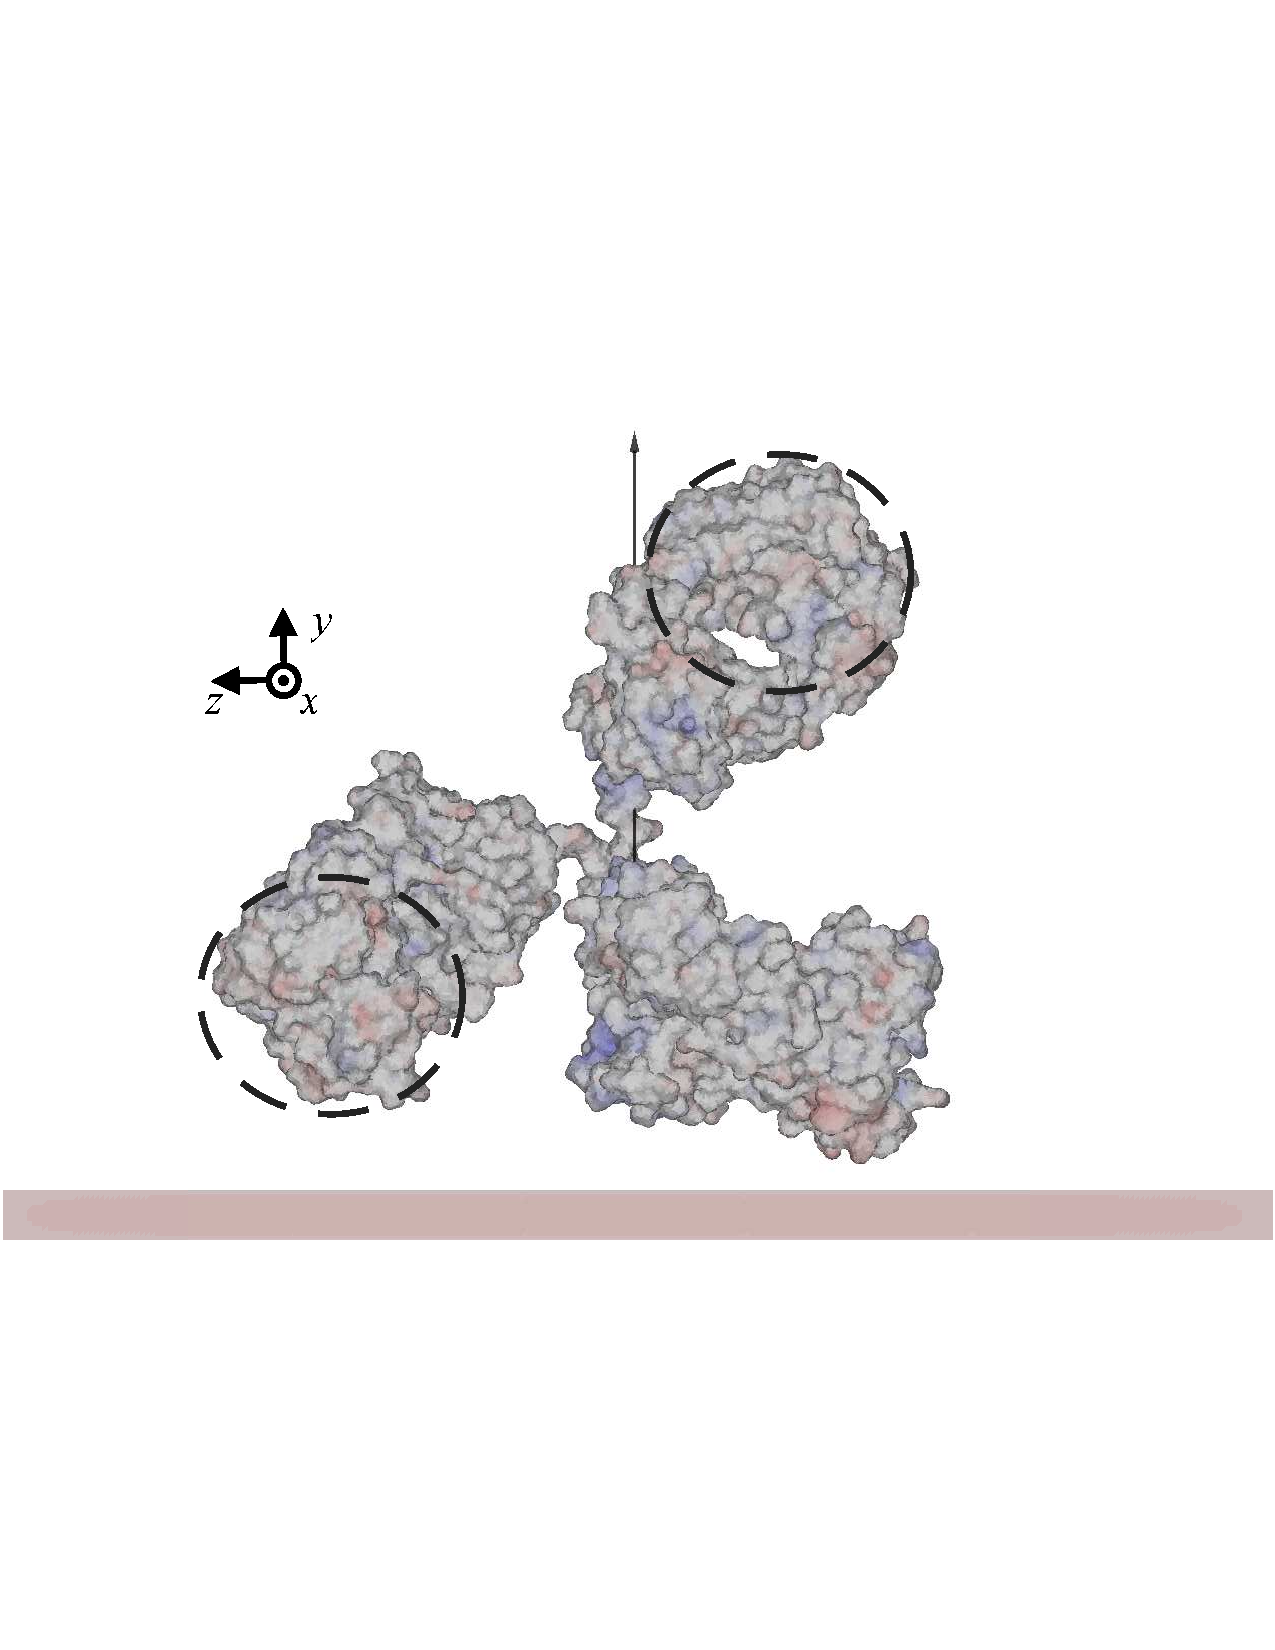
\includegraphics[width=0.4\textwidth]{Figure9d.pdf} \label{fig:1IGT_3D_sig02_kap0125_til064-rot260}}\\
   \subfloat[Probability for $\sigma$=0.05C/m$^2$ and $\kappa$=0.0625\AA$^{-1}$]{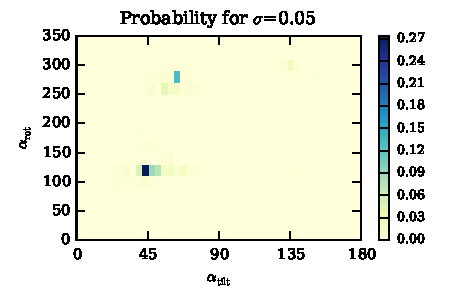
\includegraphics[width=0.4\textwidth]{Figure9e.pdf} \label{fig:1IGT_2D_sig005_kappa003125}}
   \subfloat[y-z plane view for $\alpha_{\text{tilt}} = 44^{\circ}$ and $\alpha_{\text{rot}} = 120^{\circ}$]{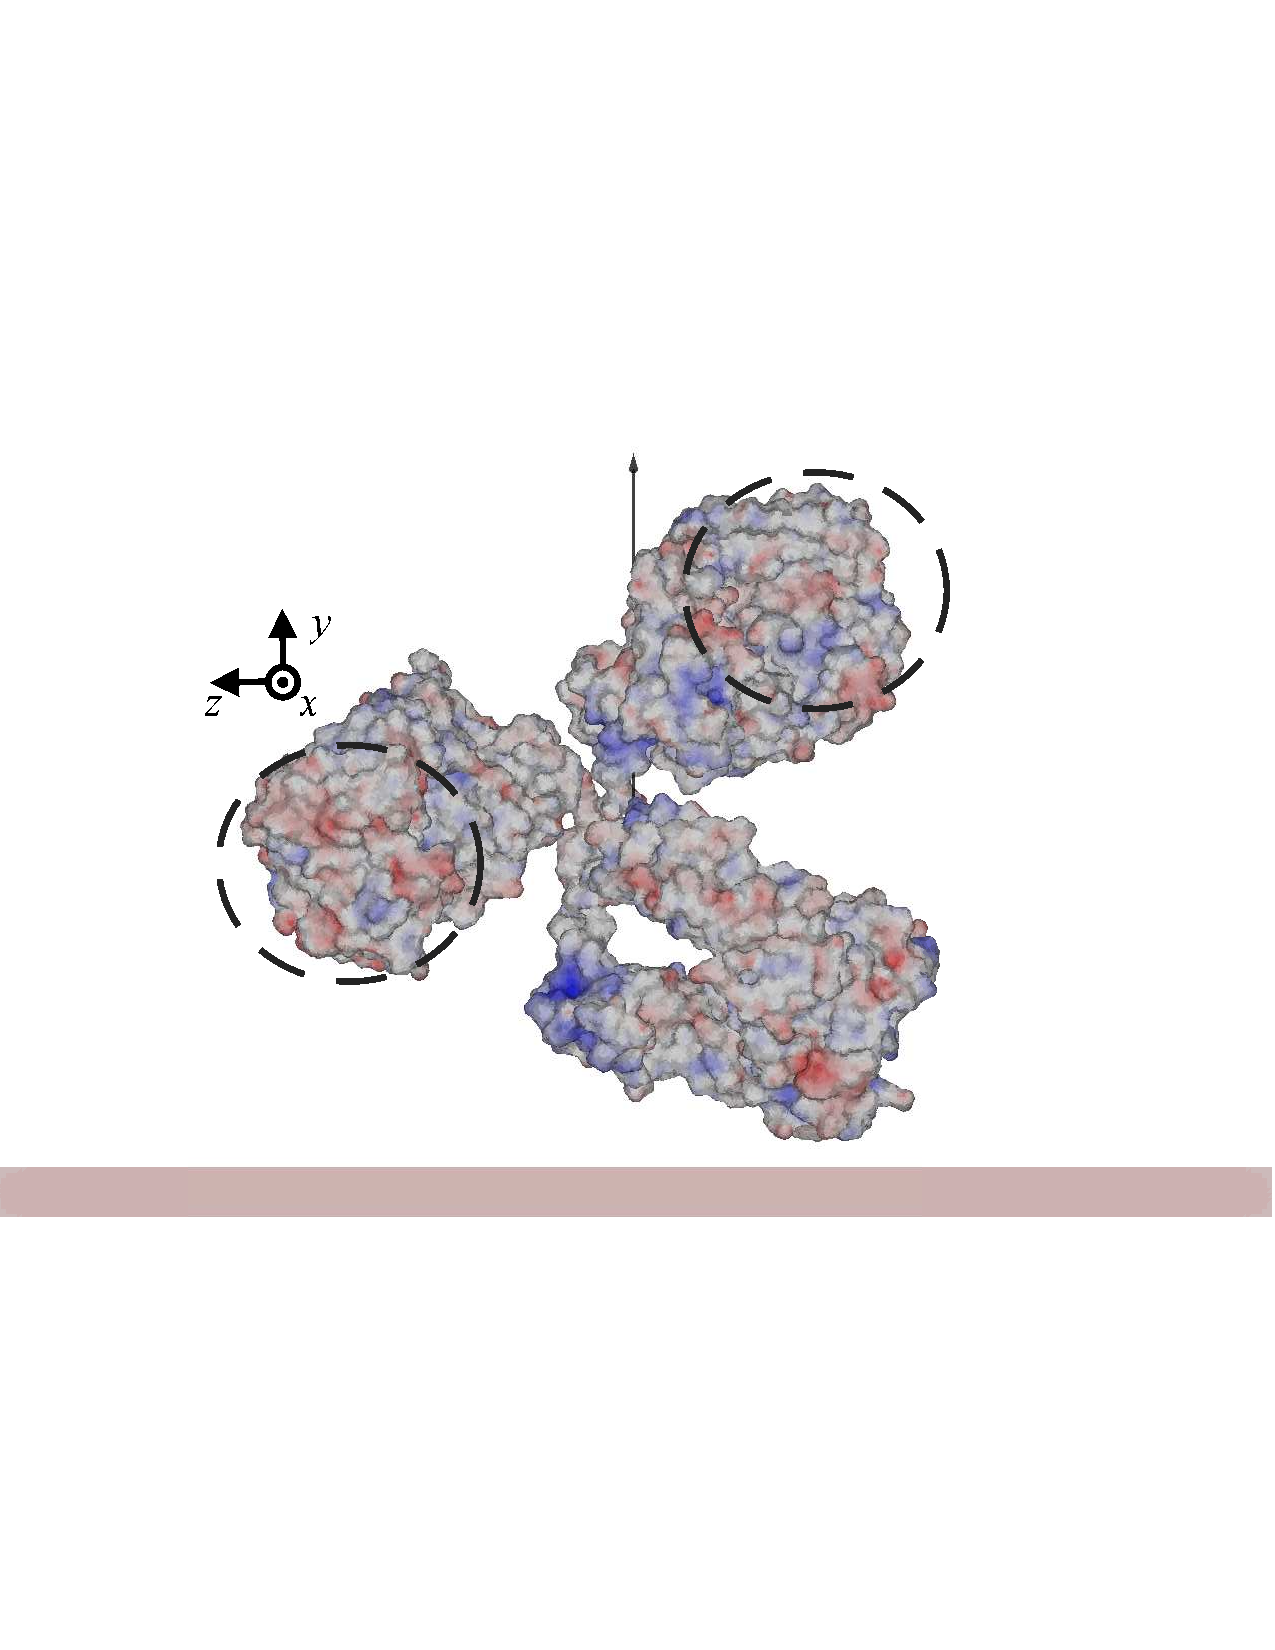
\includegraphics[width=0.4\textwidth]{Figure9f.pdf} \label{fig:1IGT_3D_sig005_kap003125_til044-rot120}}\\
   \subfloat[Probability for $\sigma$=0.1C/m$^2$ and $\kappa$=0.0625\AA$^{-1}$]{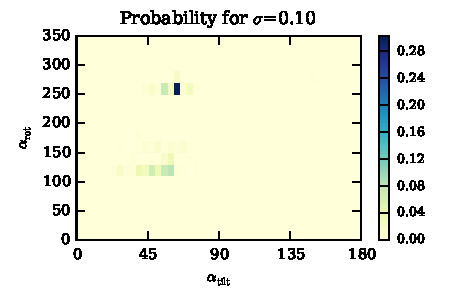
\includegraphics[width=0.4\textwidth]{Figure9g.pdf} \label{fig:1IGT_2D_sig020_kappa003125}}
   \subfloat[x-y plane view for $\alpha_{\text{tilt}} = 64^{\circ}$ and $\alpha_{\text{rot}} = 260^{\circ}$]{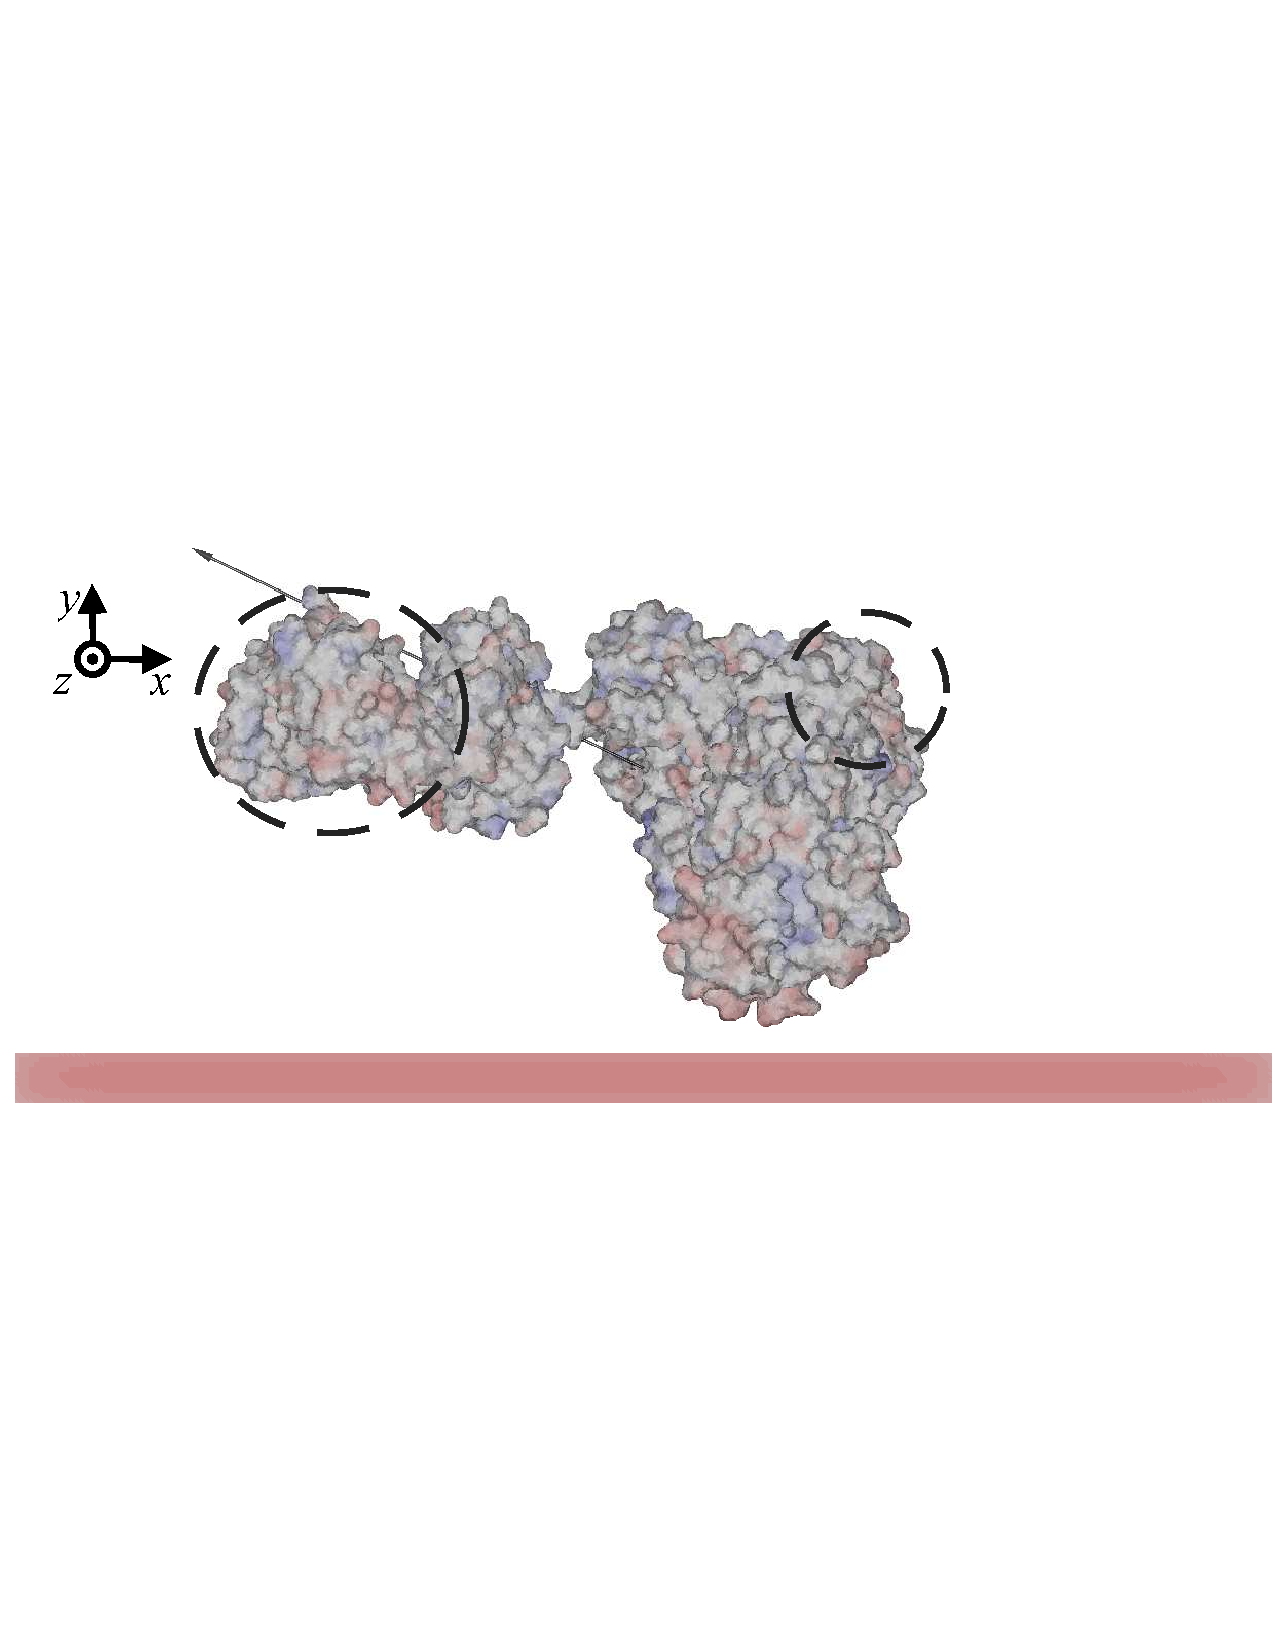
\includegraphics[width=0.4\textwidth]{Figure9h.pdf} \label{fig:1IGT_3D_sig02_kap003125_til076-rot160}}
   \caption{Orientation probability distribution and surface potential of the preferred orientation for immunoglobulin G near a positive surface charge. The black arrow indicates the direction of the dipole moment, and the circles enclose the Fab fragments. Data sets, figure files and plotting scripts available under \ccby.\cite{CooperBarba2015-share1348802}}
   \label{fig:1IGT_poscharge}
\end{figure*}